% 用 xelatex 或 latexmk -xelatex 编译
\documentclass[openany]{Template_ECNU_Undergraduate_202505/ecnuundergraduate}

\graphicspath{{./}{./Template_ECNU_Undergraduate_202505/figures/}}

\usepackage{booktabs}
\usepackage{longtable}
\usepackage{tabularx}
\usepackage{array}
\usepackage{multirow}
\usepackage{float}
\usepackage[xetex,colorlinks,breaklinks]{hyperref}
\usepackage{xurl}

\newcommand{\cvtab}[1]{\path{#1}}
\setlength{\headheight}{13pt}
\def\ctitleheading{ROGII井筒地质预测中的残差校正与模型筛选}
\def\etitleheading{Residual Correction and Model Selection for ROGII Wellbore Geology Prediction}

\begin{document}

\graduateyear{2025---2026 第二学期《统计机器学习》课程论文}
\ctitle{\uline{ROGII井筒地质预测中的\linebreak
残差校正与模型筛选}}
\etitle{\uline{Residual Correction and Model Selection\linebreak
for ROGII Wellbore Geology Prediction}}
\caffil{统计学院}
\cmajor{统计机器学习}
\csupervisor{课程组}
\academictitle{}
\cauthor{待填写}
\studentid{待填写}
\cdate{待填写}
\makecover
\clearpage

\chapter*{摘要}
\noindent 本文以 Kaggle 正式赛题 \cvtab{ROGII - Wellbore Geology Prediction} 为研究对象，讨论水平井隐藏尾段 \cvtab{TVT} 的预测问题。基于官方数据与仓库实验报告，本文首先建立尾部斜率外推的基线模型，随后在按井分组的交叉验证框架下比较了基于几何特征的残差回归模型、基于树模型的残差回归模型、学习型门控残差模型以及诊断上界。实验结果表明，基线模型的整体 RMSE 为 119.933，而基于几何特征的残差回归模型可将 RMSE 降至 15.629，并在可泛化候选中取得最佳表现；基于树模型的残差回归模型与学习型门控残差模型均优于基线，但未超过前者。简单集成与后处理未带来进一步改进。结果说明，在该任务中，稳定的数据边界、严格的交叉验证以及候选模型筛选，比单纯增加模型复杂度更为重要。

\noindent\textbf{关键词：} Kaggle；井筒地质预测；残差回归；交叉验证；模型筛选

\chapter*{Abstract}
\noindent This paper studies the TVT prediction task in the Kaggle competition \cvtab{ROGII - Wellbore Geology Prediction}. Using the official data and repository reports, we first establish a tail-slope baseline and then compare a geometry-feature residual regressor, a tree-based residual regressor, a learned gating model, and a diagnostic upper bound under well-level GroupKFold validation. The results show that the baseline reaches an overall RMSE of 119.933, while the geometry-feature residual model reduces RMSE to 15.629 and becomes the best deployable candidate. The tree-based residual model and the learned gating model both improve over the baseline but do not outperform the geometry-feature residual model. Simple blending and postprocessing do not yield further gains. These findings indicate that strict validation and candidate selection are more critical than model complexity for this task.

\noindent\textbf{Keywords:} Kaggle; wellbore prediction; residual learning; GroupKFold; model selection

\clearpage
\tableofcontents
\clearpage

\chapter{背景介绍}
ROGII 竞赛的研究对象是水平井井筒地质预测问题。参赛者需要根据井眼轨迹、已知段测井曲线以及相关参考信息，预测隐藏尾段的 \cvtab{TVT}。竞赛概览页、数据页和规则页分别为 \url{https://www.kaggle.com/competitions/rogii-wellbore-geology-prediction/overview}、\url{https://www.kaggle.com/competitions/rogii-wellbore-geology-prediction/data} 和 \url{https://www.kaggle.com/competitions/rogii-wellbore-geology-prediction/rules}。从问题形式上看，该任务既包含沿井轨迹的连续变化，也包含测井曲线形态的延续与对照，因此并不适合仅用单一静态回归方式处理。

本文采用“基线模型 + 残差回归 + 树模型比较 + 门控与筛选”的分析路线。其基本思路是先用一个稳定的外推模型提供下限，再分别考察更灵活的残差回归、树模型与门控策略是否能够在相同验证口径下带来稳定改进。全文安排如下：第二章介绍数据来源、变量含义与样本构造；第三章依次讨论基线模型、残差回归、XGBoost 以及门控、集成与模型筛选；第四章总结主要结论与经验教训。

\chapter{数据介绍}
数据来自 Kaggle 官方竞赛提供的训练集与测试集。仓库中每口训练井配有 horizontal CSV、typewell CSV 和 PNG 视觉图；公开可见测试井配有 horizontal CSV 和 typewell CSV。训练井共有 773 口，可见测试井 3 口，样例提交共有 14,151 行；训练 horizontal 的总行数为 5,092,255，训练 hidden target 行数为 3,783,989。公开可见测试集中的 3 口井与训练井重合，因此它只能用于格式核验，不能作为独立验证集。

\begin{table}[H]
\centering
\small
\begin{tabular}{@{}p{3.6cm}p{3.4cm}p{6.0cm}@{}}
\toprule
项目 & 数值 / 字段 & 说明 \\
\midrule
训练井 / 可见测试井 & 773 / 3 & 训练井用于交叉验证；可见测试井仅用于核验 \\
样例提交行数 & 14,151 & 提交格式为 \cvtab{id,tvt} \\
训练 horizontal 总行数 & 5,092,255 & 水平井原始行数总和 \\
训练 hidden target 行数 & 3,783,989 & 需要预测的隐藏尾段总行数 \\
训练 typewell 行数 & 773 & 每口训练井对应一份 typewell 文件 \\
可见测试井 ID & `000d7d20`、`00bbac68`、`00e12e8b` & 与训练井重合 \\
\bottomrule
\end{tabular}
\caption{ROGII 数据规模概览}
\end{table}

训练 horizontal 的固定列为 \cvtab{MD, X, Y, Z, ANCC, ASTNU, ASTNL, EGFDU, EGFDL, BUDA, TVT, GR, TVT\_input}；测试 horizontal 的固定列为 \cvtab{MD, X, Y, Z, GR, TVT\_input}。训练 typewell 的固定列为 \cvtab{TVT, GR, Geology}；可见测试 typewell 的固定列为 \cvtab{TVT, GR}。由此可见，\cvtab{Geology} 只存在于训练 typewell 中，训练 horizontal 的部分地层相关列也属于训练-only 信息，不能作为正式测试阶段的必需输入。

\begin{table}[H]
\centering
\small
\setlength{\tabcolsep}{4pt}
\renewcommand{\arraystretch}{0.95}
\begin{tabularx}{0.95\textwidth}{@{}p{2.2cm}X@{}}
\toprule
字段 & 含义 / 作用 \\
\midrule
\cvtab{MD} & 测深或井深索引，用于表示沿井轨迹的采样位置 \\
\cvtab{X}, \cvtab{Y}, \cvtab{Z} & 井轨迹空间坐标，用于描述轨迹几何形态 \\
\cvtab{GR} & 自然伽马测井曲线，反映测井响应 \\
\cvtab{TVT} & 预测目标，即真实 \cvtab{TVT} 值 \\
\cvtab{TVT\_input} & 预测起点之前的已知 \cvtab{TVT} 段；隐藏尾段对应位置缺失 \\
\cvtab{ANCC} & 训练-only 地层相关列 \\
\cvtab{ASTNU} & 训练-only 地层相关列 \\
\cvtab{ASTNL} & 训练-only 地层相关列 \\
\cvtab{EGFDU} & 训练-only 地层相关列 \\
\cvtab{EGFDL} & 训练-only 地层相关列 \\
\cvtab{BUDA} & 训练-only 地层相关列 \\
\cvtab{Geology} & typewell 训练标签；测试集中不存在 \\
\bottomrule
\end{tabularx}
\caption{主要字段说明}
\end{table}

\chapter{数据分析}

\section{数据预处理与描述统计}
在建模之前，首先需要确认训练集、测试集与提交格式在字段层面的对应关系。仓库中的样本统计显示，训练 horizontal 的每井长度分布较宽，平均 6,587.650 行，中位数 6,576 行，最短 2,058 行，最长 12,141 行。公开可见测试井分别有 5,278、7,559 和 6,384 行，而需要预测的尾段分别为 3,836、6,014 和 4,301 行。训练 horizontal 中 \cvtab{GR} 的缺失率为 29.610\%，\cvtab{TVT\_input} 的缺失率为 74.310\%，与“前段已知、后段隐藏”的任务形态一致。

\begin{table}[H]
\centering
\small
\begin{tabular}{@{}p{5.1cm}p{3.1cm}p{6.1cm}@{}}
\toprule
指标 & 数值 & 说明 \\
\midrule
训练 horizontal 每井 rows mean / std / min / median / max & 6,587.650 / 1,311.460 / 2,058 / 6,576 / 12,141 & 原始水平井长度分布较宽 \\
公开可见测试井 rows & 5,278 / 7,559 / 6,384 & 仅用于格式与一致性核验 \\
公开可见测试井 target rows & 3,836 / 6,014 / 4,301 & 公开可见尾段长度 \\
训练 horizontal GR missing rate & 29.610\% & GR 缺失较多 \\
训练 horizontal TVT\_input missing rate & 74.310\% & 与隐藏尾段对应 \\
target rows min / median / max & 407 / 4,840 / 10,052 & 隐藏尾段长度跨度大 \\
known rows min / median / max & 851 / 1,703 / 2,392 & 已知段长度相对较短 \\
\bottomrule
\end{tabular}
\caption{ROGII 原始数据的描述统计}
\end{table}

typewell 的 \cvtab{Geology} 标签分布显著不均衡，最大类 \cvtab{ANCC} 为 294,268，最小类 \cvtab{EGFD200} 仅为 1。该分布表明，\cvtab{Geology} 更适合作为训练诊断或辅助分析变量，而不宜作为测试阶段的硬性输入。另一方面，隐藏尾段越长，基线模型误差越大；在 4k 行以上的尾段区间，基线的平均 RMSE 明显上升。

\begin{table}[H]
\centering
\small
\begin{tabular}{@{}p{4.6cm}p{2.4cm}p{2.4cm}p{4.4cm}@{}}
\toprule
target rows bucket & wells & mean RMSE & 说明 \\
\midrule
0-2k & 6 & 9.709 & 最短尾段区间，基线尚可 \\
2k-4k & 178 & 30.137 & 误差开始明显增加 \\
4k-6k & 447 & 57.833 & 主体区间，基线难度显著上升 \\
6k-8k & 128 & 91.024 & 长尾段区间，误差进一步放大 \\
8k-12k & 14 & 122.556 & 最难区间，基线表现最差 \\
\bottomrule
\end{tabular}
\caption{基线模型在不同隐藏尾段长度上的表现}
\end{table}

\section{基线模型}
基线模型采用尾部斜率外推，其作用在于为后续模型提供稳定的对照组和性能下限。记基线预测为 \(\hat y_{\mathrm{base}}\)，则其本质上是利用已知段 \cvtab{TVT\_input} 的趋势，对隐藏尾段进行延续性外推。虽然这种方法没有显式利用复杂的地层结构，但它具有可解释、稳定和易于复现的优点。

\begin{table}[H]
\centering
\small
\begin{tabular}{@{}p{3.5cm}p{1.9cm}p{1.7cm}p{1.7cm}p{1.9cm}p{1.9cm}@{}}
\toprule
指标 & RMSE & MAE & P95 abs error & 最大绝对误差 & 说明 \\
\midrule
基线模型 & 119.933 & 53.680 & 182.780 & 2552.660 & 对照组 \\
\bottomrule
\end{tabular}
\caption{基线模型的整体表现}
\end{table}

从分段结果看，基线模型在短尾段上误差较小，但当隐藏尾段长度增加时，误差迅速增大，说明单纯依赖尾部外推并不足以覆盖较长的结构延续区间。

\section{残差回归}
残差回归的核心思想是先由基线模型给出一个初始预测，再对基线误差进行二次建模。若记真实值为 \(y\)，基线预测为 \(\hat y_{\mathrm{base}}\)，则残差目标可写为

\[
r = y - \hat y_{\mathrm{base}},
\qquad
\hat y = \hat y_{\mathrm{base}} + \hat r(x).
\]

其中，\(x\) 表示可用于测试阶段的几何信息、已知段长度、\cvtab{GR} 缺失结构及若干滚动统计量。基于几何特征的残差回归模型采用标准化后的线性回归器，其主要参数为 \(\alpha=0.0005\)、\(\texttt{max\_iter}=30\)、\(\texttt{tol}=10^{-3}\)、\(\texttt{early\_stopping}=True\)、\(\texttt{validation\_fraction}=0.1\)、\(\texttt{n\_iter\_no\_change}=3\) 与 \(\texttt{average}=True\)。该模型在训练井上按井分组进行交叉验证，避免同一口井同时出现在训练与验证两侧。

\begin{table}[H]
\centering
\small
\begin{tabular}{@{}p{4.5cm}p{2.2cm}p{1.6cm}p{1.6cm}p{1.8cm}p{1.8cm}@{}}
\toprule
方法 & 角色 & RMSE & MAE & P95 abs error & 改善 / 退化井 \\
\midrule
基线模型 & 对照组 & 119.933 & 53.680 & 182.780 & - \\
基于几何特征的残差回归模型 & 线性残差回归 & 15.629 & 11.173 & 31.945 & 632 / 141 \\
\bottomrule
\end{tabular}
\caption{基线模型与基于几何特征的残差回归模型比较}
\end{table}

从结果看，基于几何特征的残差回归模型将 RMSE 从 119.933 降至 15.629，说明在相同验证口径下，残差建模显著优于单纯外推。与此同时，仍有 141 口井出现退化，表明残差回归不能无条件替代基线，而应与基线共同构成候选比较体系。

\section{XGBoost}
XGBoost 属于梯度提升树模型，能够通过逐步叠加弱学习器捕捉非线性关系和特征交互。与线性残差回归相比，树模型理论上具有更强的拟合能力，但也更依赖特征信息的完整性以及样本结构的稳定性。本文仍然保持相同的残差目标，即以 \(y-\hat y_{\mathrm{base}}\) 作为监督信号，再在相同的按井分组交叉验证框架下进行比较。

\begin{table}[H]
\centering
\small
\begin{tabular}{@{}p{4.0cm}p{10.5cm}@{}}
\toprule
方法 & 关键设置 \\
\midrule
基于树模型的残差回归模型 & \(\texttt{n\_estimators}=30\)、\(\texttt{max\_depth}=4\)、\(\texttt{learning\_rate}=0.05\)、\(\texttt{subsample}=0.9\)、\(\texttt{colsample\_bytree}=0.9\)、\(\texttt{reg\_lambda}=1.0\)、\(\texttt{tree\_method}=\texttt{hist}\)、\(\texttt{n\_jobs}=1\) \\
\bottomrule
\end{tabular}
\caption{基于树模型的残差回归模型参数设置}
\end{table}

\begin{table}[H]
\centering
\small
\begin{tabular}{@{}p{4.5cm}p{2.2cm}p{1.6cm}p{1.6cm}p{1.8cm}p{1.8cm}@{}}
\toprule
方法 & 角色 & RMSE & MAE & P95 abs error & 改善 / 退化井 \\
\midrule
基线模型 & 对照组 & 119.933 & 53.680 & 182.780 & - \\
基于几何特征的残差回归模型 & 线性残差回归 & 15.629 & 11.173 & 31.945 & 632 / 141 \\
基于树模型的残差回归模型 & 树残差回归 & 31.473 & 13.748 & 34.654 & 626 / 147 \\
\bottomrule
\end{tabular}
\caption{树模型与线性残差回归模型比较}
\end{table}

从交叉验证结果看，基于树模型的残差回归模型优于基线模型，但明显弱于基于几何特征的残差回归模型。结合当前特征信息与样本结构可以看出，树模型虽然复杂度更高，但并未自动带来更优结果，说明在该任务中模型复杂度必须与特征质量和验证表现相匹配。

\section{门控、集成与模型筛选}
门控模型可写为

\[
\hat y = \hat y_{\mathrm{base}} + \hat \alpha(x)\hat r(x),
\]

其中 \(\hat \alpha(x)\) 表示对残差的信任程度。学习型门控残差模型通过回归方式学习 \(\alpha\)，其交叉验证预测 RMSE 为 19.818，优于基线，但仍未超过基于几何特征的残差回归模型。诊断上界则通过每口训练井自身的真值搜索最佳 \(\alpha\)，其 RMSE 为 13.381；由于该过程依赖同井真值，因此只能作为上界分析，不能作为最终泛化模型。

\begin{table}[H]
\centering
\small
\begin{tabular}{@{}p{4.8cm}p{2.0cm}p{7.0cm}@{}}
\toprule
候选 & RMSE & 说明 \\
\midrule
基于几何特征的残差回归模型 & 15.629 & 最终可泛化候选 \\
学习型门控残差模型 & 19.818 & 可泛化门控候选 \\
诊断上界 & 13.381 & 仅作上界分析 \\
\bottomrule
\end{tabular}
\caption{门控模型比较}
\end{table}

集成结果显示，简单组合并未优于基于几何特征的残差回归模型：\cvtab{optimized} 与该模型持平，而 \cvtab{balanced}、\cvtab{aggressive} 和 \cvtab{conservative} 均明显恶化。

\begin{table}[H]
\centering
\small
\begin{tabular}{@{}p{4.2cm}p{2.0cm}p{7.0cm}@{}}
\toprule
候选 & RMSE & 说明 \\
\midrule
基于几何特征的残差回归模型 & 15.629 & 基准候选 \\
\cvtab{optimized} & 15.629 & 与基准候选持平 \\
\cvtab{balanced} & 42.223 & 明显劣化 \\
\cvtab{aggressive} & 59.901 & 明显劣化 \\
\cvtab{conservative} & 109.595 & 明显劣化 \\
\bottomrule
\end{tabular}
\caption{集成候选的交叉验证结果}
\end{table}

候选模型筛选时，先以基线模型的覆盖范围为参照，要求候选的行覆盖率和井覆盖率均不低于 95\%；随后在满足覆盖条件的候选中按完整覆盖下的交叉验证预测 RMSE 排序。若候选之间的差异落在 0.01 的容忍区间内，则进一步比较最差井 RMSE、退化井数量与 P95 绝对误差。最终被选中的候选是基于几何特征的残差回归模型，其覆盖率与基线完全一致（1.000 / 1.000），且交叉验证预测 RMSE 最低。

后处理同样需要遵循交叉验证约束。仓库中的后处理候选将 RMSE 从 15.629 恶化到 69.926，因此未被采纳。

\begin{table}[H]
\centering
\small
\begin{tabular}{@{}p{4.5cm}p{2.4cm}p{2.4cm}p{3.8cm}@{}}
\toprule
候选 & RMSE before & RMSE after & 结论 \\
\midrule
后处理候选 & 15.629 & 69.926 & 拒绝 \\
\bottomrule
\end{tabular}
\caption{后处理结果}
\end{table}

\chapter{结论}
本文围绕 ROGII 井筒地质预测任务，基于官方资料与仓库实验报告，对尾部外推基线、残差回归、树模型、门控、集成与模型筛选进行了统一比较。结果表明，在当前任务设定下，最有效的策略并不是单纯提高模型复杂度，而是先建立可审计的基线模型，再在按井分组的交叉验证框架下验证残差修正是否真正带来稳定改进。就可泛化候选而言，基于几何特征的残差回归模型表现最佳，并被筛选为最终候选；基于树模型的残差回归模型与学习型门控残差模型可作为对照，但并未超过前者。

结合交叉验证和结果对比可以看出，XGBoost 虽然具有更强的非线性拟合能力，但在当前特征信息和样本结构下并未优于结构更简单的残差回归模型。这一结果提示，在类似的井筒预测任务中，模型复杂度不应被视为提升性能的充分条件，而应结合数据规模、结构特征与验证结果进行选择。对于本研究而言，更有价值的经验是：首先保证验证边界清晰，其次再讨论模型表达能力是否足够。

\chapter*{附录}
\addcontentsline{toc}{chapter}{附录}

\section*{A. 数据与任务说明}
\noindent 本节汇总可直接复核正文的数据与任务定义。
\begin{itemize}
  \item 官方竞赛页面：\url{https://www.kaggle.com/competitions/rogii-wellbore-geology-prediction/overview}
  \item 官方数据页面：\url{https://www.kaggle.com/competitions/rogii-wellbore-geology-prediction/data}
  \item 官方规则页面：\url{https://www.kaggle.com/competitions/rogii-wellbore-geology-prediction/rules}
\end{itemize}

\begin{table}[H]
\centering
\small
\begin{tabularx}{0.97\textwidth}{@{}p{3.0cm}p{3.6cm}p{3.6cm}X@{}}
\toprule
项目 & 训练集 & 测试集 & 说明 \\
\midrule
Horizontal 主列 & \cvtab{MD, X, Y, Z, ANCC, ASTNU, ASTNL, EGFDU, EGFDL, BUDA, TVT, GR, TVT\_input} & \cvtab{MD, X, Y, Z, GR, TVT\_input} & 训练集额外包含地层相关列和真值 \\
Typewell 主列 & \cvtab{TVT, GR, Geology} & \cvtab{TVT, GR} & \cvtab{Geology} 仅存在于训练 typewell \\
训练-only 字段 & \cvtab{ANCC, ASTNU, ASTNL, EGFDU, EGFDL, BUDA} & 无 & 不能作为正式测试阶段的必需输入 \\
评价与提交 & RMSE；\cvtab{id,tvt} & RMSE；\cvtab{id,tvt} & \cvtab{id = well\_row\_index} \\
\bottomrule
\end{tabularx}
\caption{数据与任务说明补充}
\end{table}

\noindent 公开可见测试集与训练集重合，因此只能用于格式核验与脚本一致性检查，不应作为独立验证集。

\section*{B. 数据统计与任务难点}
\noindent 下面的统计用于支撑正文对任务难点的判断。

\begin{table}[H]
\centering
\small
\begin{tabularx}{0.97\textwidth}{@{}p{5.0cm}p{3.2cm}X@{}}
\toprule
统计项 & 数值 & 说明 \\
\midrule
训练 horizontal 每井 rows mean / std / min / median / max & 6,587.650 / 1,311.460 / 2,058 / 6,576 / 12,141 & 原始水平井长度分布较宽 \\
公开可见测试井 rows & 5,278 / 7,559 / 6,384 & 仅用于格式与一致性核验 \\
公开可见测试井 target rows & 3,836 / 6,014 / 4,301 & 公开可见尾段长度 \\
训练 horizontal GR missing rate & 29.610\% & GR 缺失较多 \\
训练 horizontal TVT\_input missing rate & 74.310\% & 与隐藏尾段对应 \\
训练 horizontal ANCC missing rate & 0.900\% & 训练-only 地层列少量缺失 \\
训练 horizontal EGFDL missing rate & 0.120\% & 训练-only 地层列少量缺失 \\
target rows min / median / max & 407 / 4,840 / 10,052 & 隐藏尾段长度跨度大 \\
known rows min / median / max & 851 / 1,703 / 2,392 & 已知段长度相对较短 \\
target GR missing q0 / q25 / q50 / q75 / q90 / max & 0.0067 / 0.1308 / 0.3029 / 0.4977 / 0.5946 / 0.8118 & 目标段 GR 缺失率分布 \\
\bottomrule
\end{tabularx}
\caption{数据统计补充}
\end{table}

\begin{table}[H]
\centering
\small
\begin{tabularx}{0.97\textwidth}{@{}p{4.8cm}p{2.4cm}p{2.4cm}X@{}}
\toprule
label & count & 位置 & 说明 \\
\midrule
ANCC & 294,268 & 最多 & typewell 标签最常见类别 \\
EGFDL & 205,397 & 较多 & 次高频类别 \\
ASTNL & 172,223 & 较多 & 高频类别 \\
BUDA & 140,640 & 较多 & 高频类别 \\
ASTNU & 118,025 & 较多 & 高频类别 \\
EGFDU & 70,013 & 较多 & 高频类别 \\
EGFD200 & 1 & 最少 & 极端稀有类别 \\
\bottomrule
\end{tabularx}
\caption{typewell Geology 类别分布补充}
\end{table}

\begin{table}[H]
\centering
\small
\begin{tabular}{@{}p{3.4cm}p{1.8cm}p{2.0cm}p{2.0cm}p{2.0cm}@{}}
\toprule
target rows bucket & wells & mean RMSE & median RMSE & max RMSE \\
\midrule
0-2k & 6 & 9.709 & 9.617 & 17.739 \\
2k-4k & 178 & 30.137 & 21.488 & 114.625 \\
4k-6k & 447 & 57.833 & 39.775 & 1465.970 \\
6k-8k & 128 & 91.024 & 47.382 & 1434.250 \\
8k-12k & 14 & 122.556 & 119.480 & 264.742 \\
\bottomrule
\end{tabular}
\caption{基线模型在不同隐藏尾段长度上的表现}
\end{table}

\section*{C. 完整实验结果}
\noindent 下表汇总可泛化候选与诊断上界的完整交叉验证结果。

\begin{table}[H]
\centering
\small
\begin{tabular}{@{}p{4.7cm}p{1.8cm}p{1.8cm}p{2.0cm}p{2.0cm}@{}}
\toprule
方法 & RMSE & MAE & P95 abs error & 退化井数 \\
\midrule
基线模型 & 119.933 & 53.680 & 182.780 & - \\
基于几何特征的残差回归模型 & 15.629 & 11.173 & 31.945 & 141 \\
基于树模型的残差回归模型 & 31.473 & 13.748 & 34.654 & 147 \\
学习型门控残差模型 & 19.818 & 13.984 & 41.698 & 120 \\
诊断上界 & 13.381 & 9.468 & 27.353 & 0 \\
\bottomrule
\end{tabular}
\caption{主要候选模型的完整交叉验证结果}
\end{table}

\begin{table}[H]
\centering
\small
\begin{tabular}{@{}p{2.0cm}p{2.0cm}p{2.0cm}p{2.0cm}p{2.2cm}@{}}
\toprule
alpha & RMSE & MAE & P95 abs error & 说明 \\
\midrule
1.00 & 15.6288 & 11.1732 & 31.9450 & 选定值 \\
0.75 & 33.6079 & 18.2440 & 57.6606 & 明显变差 \\
0.50 & 61.4914 & 29.3052 & 97.7526 & 明显变差 \\
0.25 & 90.5503 & 41.2999 & 140.5640 & 明显变差 \\
0.00 & 119.9330 & 53.6804 & 182.7800 & 退化为基线 \\
\bottomrule
\end{tabular}
\caption{几何残差模型的 alpha 搜索结果}
\end{table}

\begin{table}[H]
\centering
\small
\begin{tabular}{@{}p{4.2cm}p{1.8cm}p{2.2cm}p{2.2cm}p{2.0cm}@{}}
\toprule
候选 & RMSE before & RMSE after & 结论 & 说明 \\
\midrule
geometry & 15.629 & 69.926 & 拒绝 & 后处理护栏失败 \\
optimized & 15.629 & 15.629 & 持平 & 与 geometry 持平 \\
balanced & 42.223 & - & 变差 & 不优于 geometry \\
aggressive & 59.901 & - & 变差 & 不优于 geometry \\
conservative & 109.595 & - & 变差 & 不优于 geometry \\
\bottomrule
\end{tabular}
\caption{集成与后处理的完整比较}
\end{table}

\section*{D. 候选筛选与失败案例}
\noindent 候选筛选先以 baseline 覆盖范围为参照，正式排名要求行覆盖率和井覆盖率均不低于 95\%；排序依据完整覆盖下的 OOF RMSE。若候选差异落在 0.01 容忍区间内，则进一步比较最差井 RMSE、退化井数量与 P95 abs error。后处理仅在 OOF 改善时保留，诊断上界不参与自动选择。

\begin{table}[H]
\centering
\small
\begin{tabularx}{0.97\textwidth}{@{}p{3.7cm}p{2.3cm}p{2.1cm}p{2.2cm}X@{}}
\toprule
候选 & 状态 & OOF RMSE & 覆盖率 & 说明 \\
\midrule
geometry & selected & 15.6288 & 1.000 / 1.000 & 完整覆盖下 RMSE 最低 \\
xgb & valid & 31.4731 & 1.000 / 1.000 & 可泛化但不优于 geometry \\
learned\_gated\_geometry & valid & 19.8180 & 1.000 / 1.000 & 可泛化但不优于 geometry \\
gated\_geometry & skipped & 13.3807 & 1.000 / 1.000 & 诊断上界，自动选择中排除 \\
geometry\_postprocessed & rejected & 69.9255 & 1.000 / 1.000 & 后处理护栏失败 \\
\bottomrule
\end{tabularx}
\caption{候选筛选结果补充}
\end{table}

\begin{table}[H]
\centering
\small
\begin{tabular}{@{}p{2.1cm}p{1.5cm}p{1.9cm}p{2.0cm}p{2.0cm}@{}}
\toprule
well & rows & RMSE & baseline RMSE & 相对 baseline \\
\midrule
1b1eba53 & 4,655 & 69.3534 & 21.9863 & -47.3672 \\
86454a6f & 7,964 & 64.3403 & 29.6178 & -34.7225 \\
5f4d2a52 & 5,225 & 59.4918 & 116.7140 & 57.2222 \\
2fd68f7b & 4,730 & 58.8138 & 113.3370 & 54.5234 \\
ba48188d & 4,166 & 52.9596 & 74.5768 & 21.6172 \\
f88ddb26 & 4,990 & 51.8977 & 24.2101 & -27.6876 \\
fef8af96 & 3,826 & 48.1773 & 110.5840 & 62.4067 \\
43e16325 & 3,720 & 44.2896 & 45.7767 & 1.4871 \\
\bottomrule
\end{tabular}
\caption{候选筛选后最差井的典型样例}
\end{table}

\section*{E. 图表附录}
\noindent 下列图像直接对应报告中的代表性井段，用于说明模型在极端样本上的行为。

\clearpage
\begin{figure}[p]
\centering
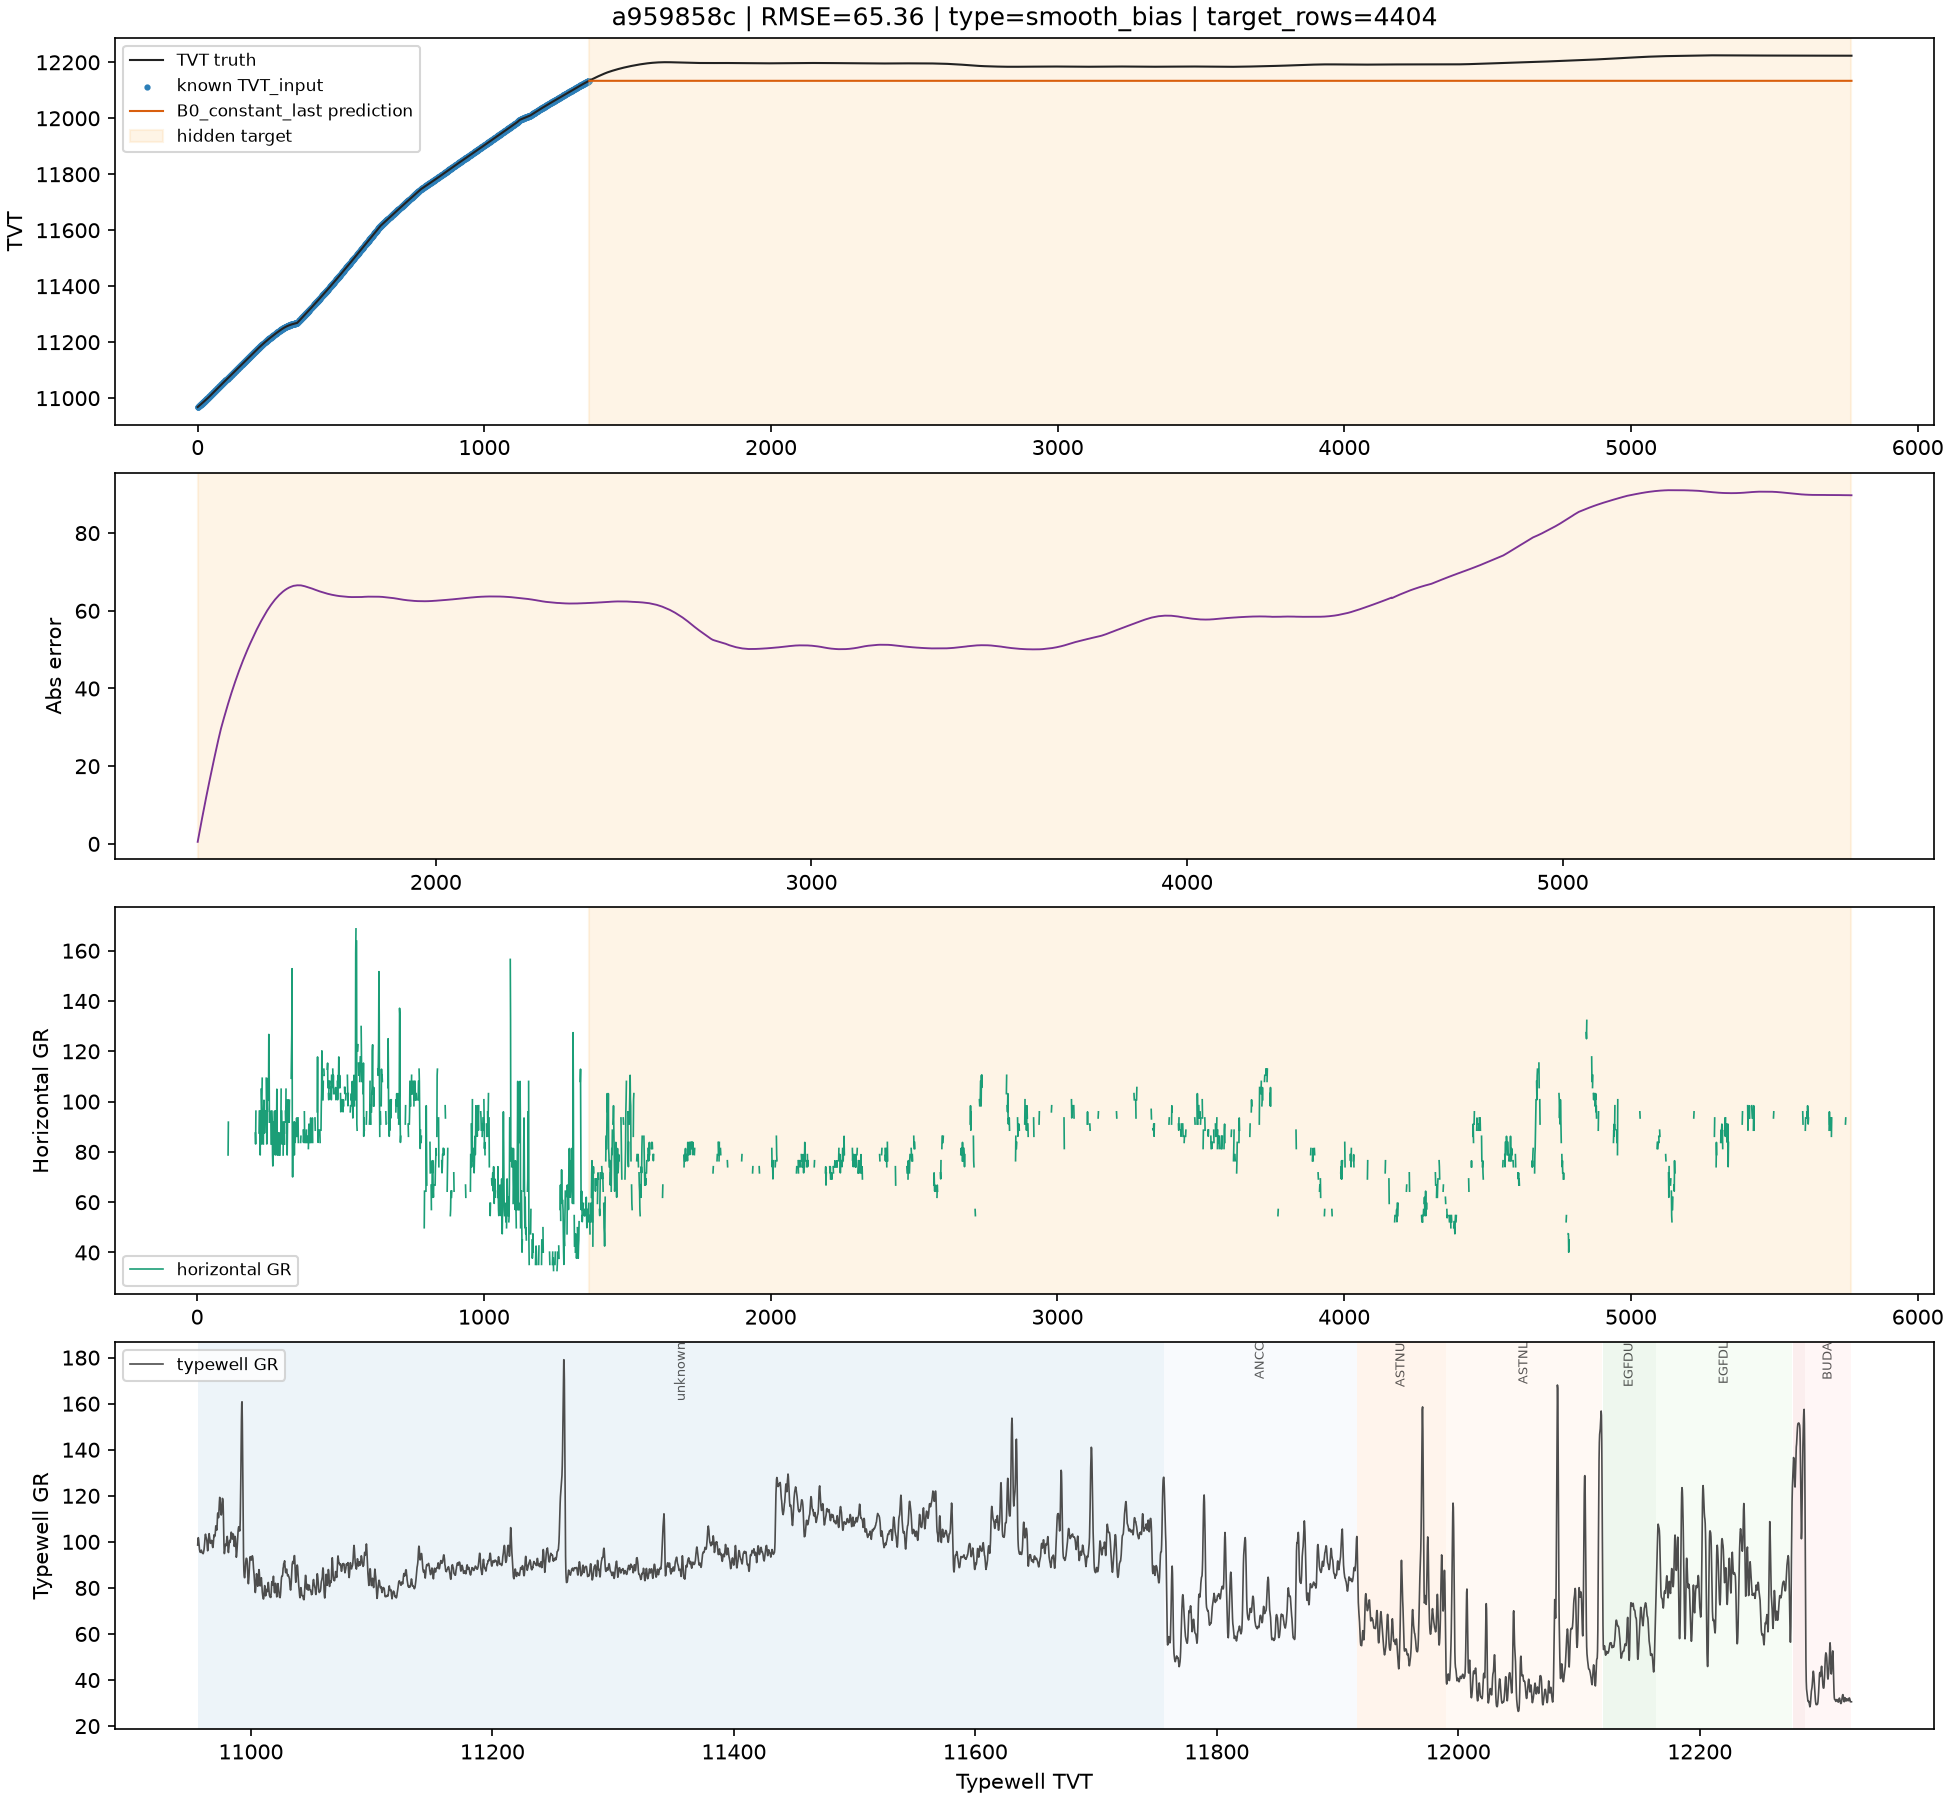
\includegraphics[width=0.95\textwidth,height=0.76\textheight,keepaspectratio]{../../reports/figures/baseline_worst_wells/03_a959858c.png}
\caption{基线最差井示例：`a959858c`}
\end{figure}

\clearpage
\begin{figure}[p]
\centering
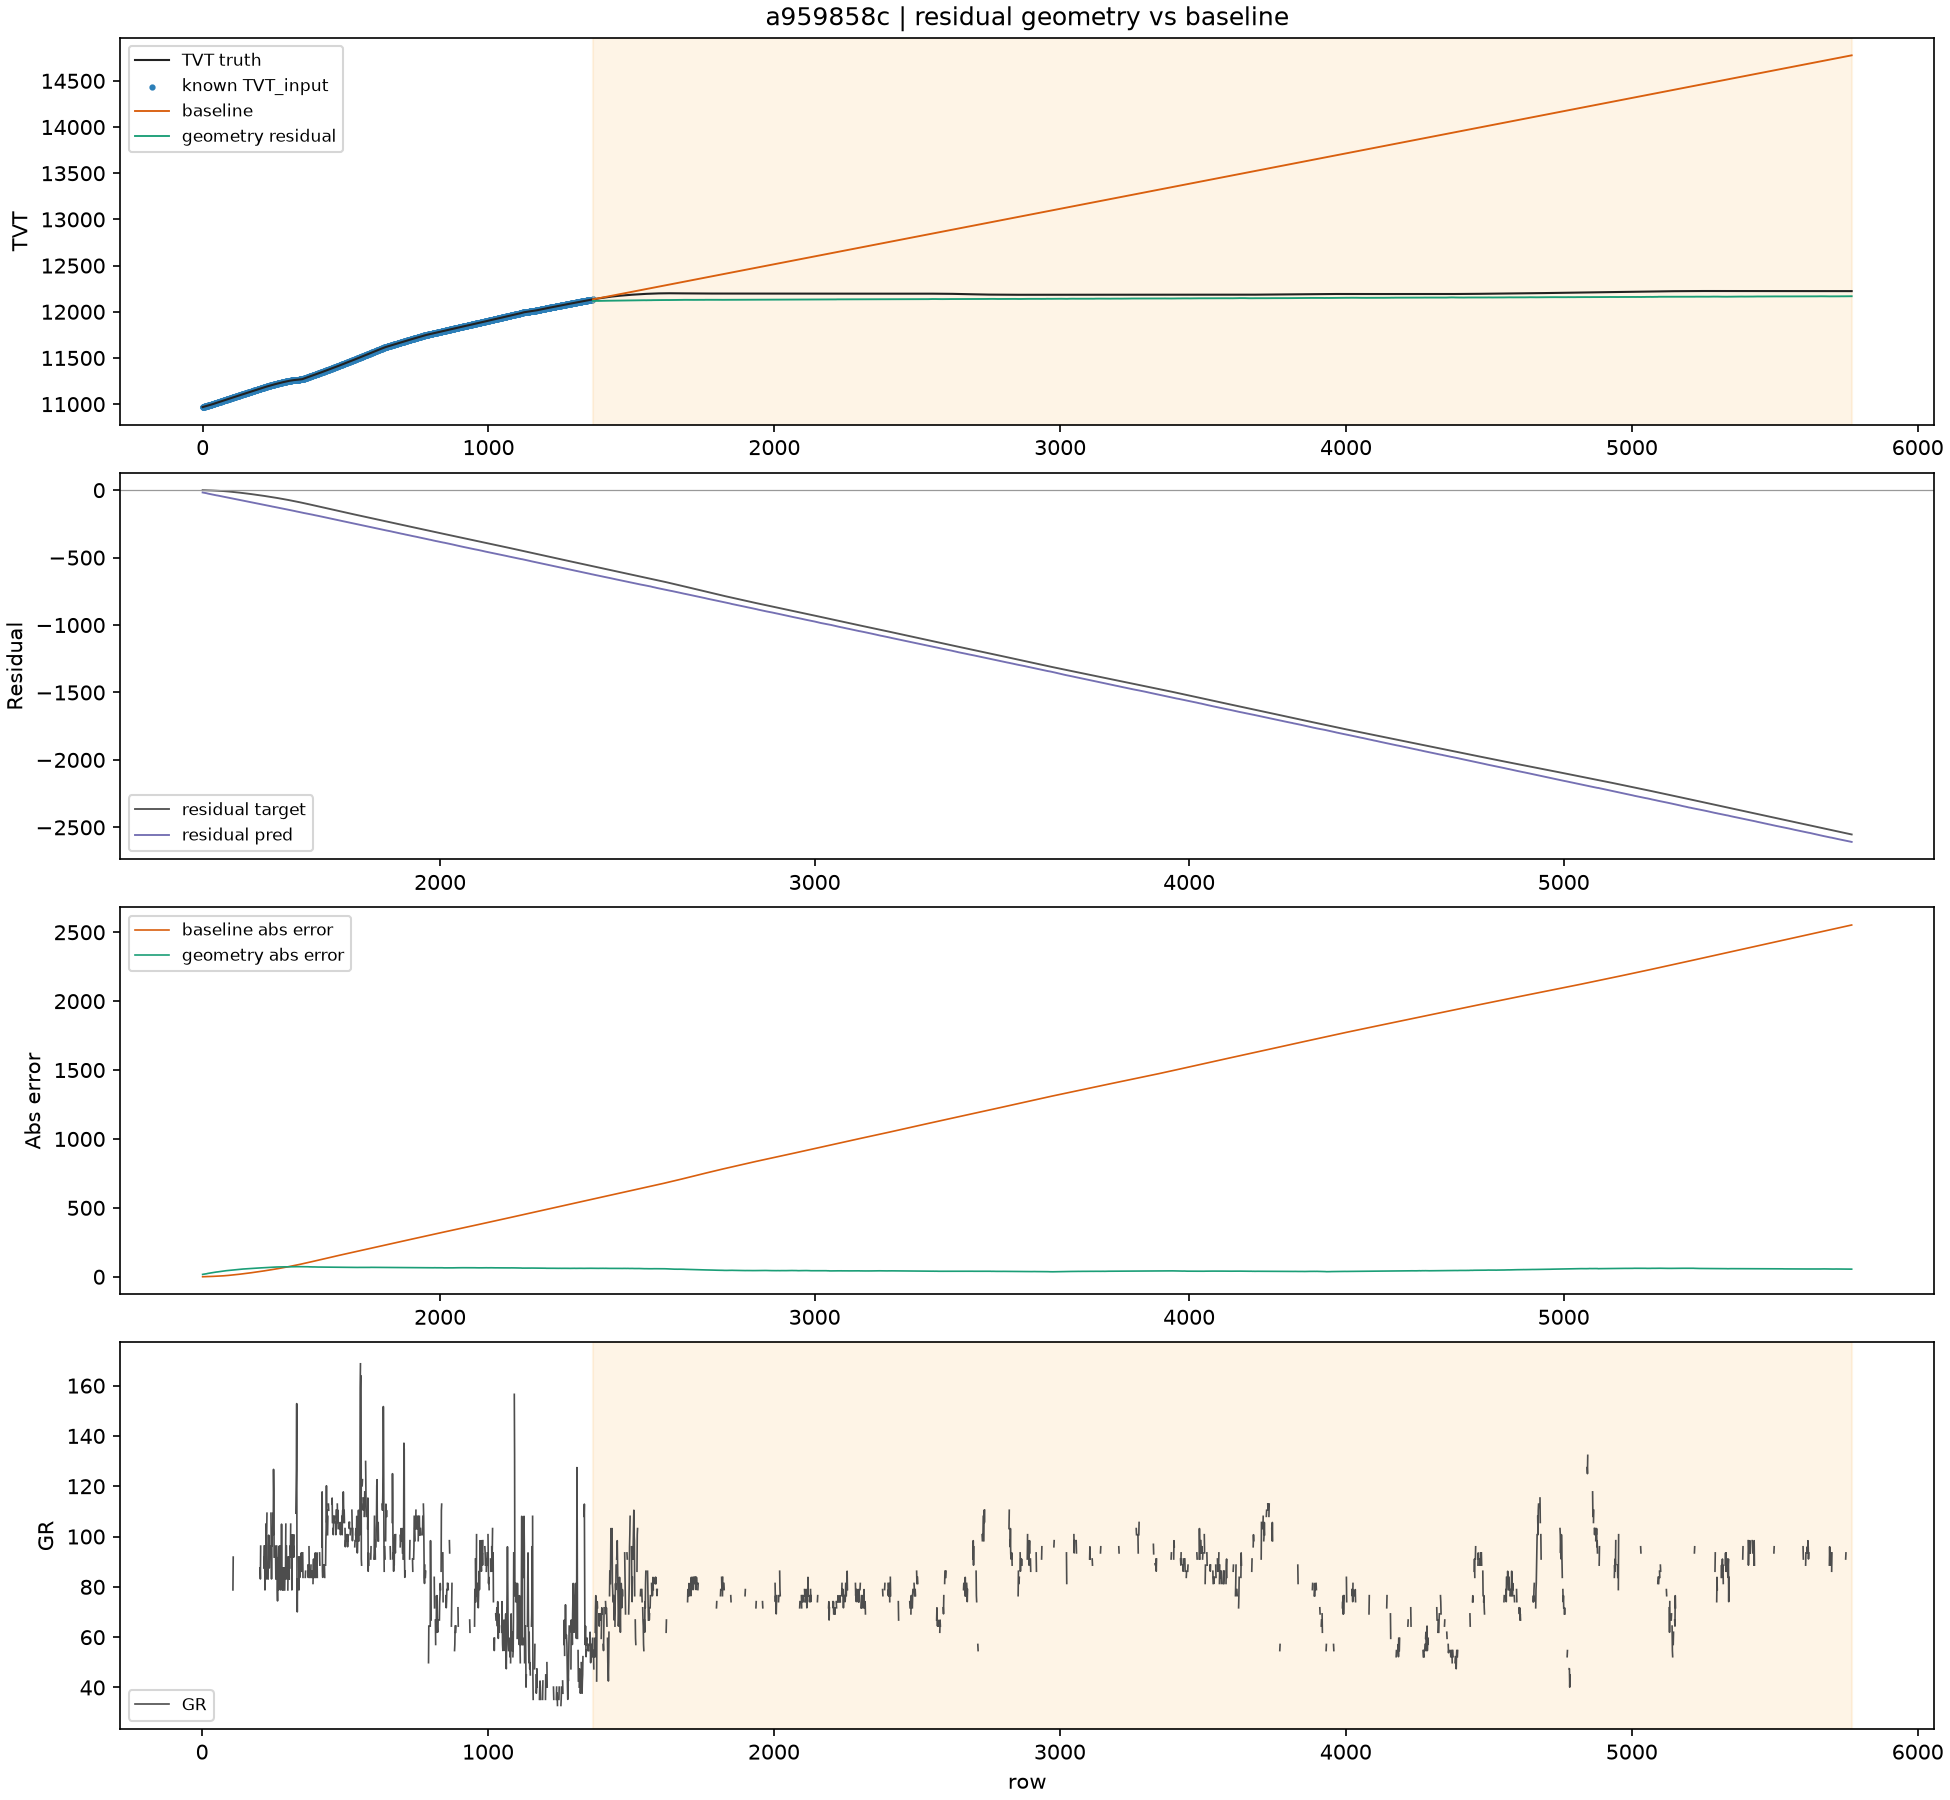
\includegraphics[width=0.95\textwidth,height=0.76\textheight,keepaspectratio]{../../reports/figures/residual_geometry_best_improved/01_a959858c.png}
\caption{几何残差模型最佳改进井示例：`a959858c`}
\end{figure}

\clearpage
\begin{figure}[p]
\centering
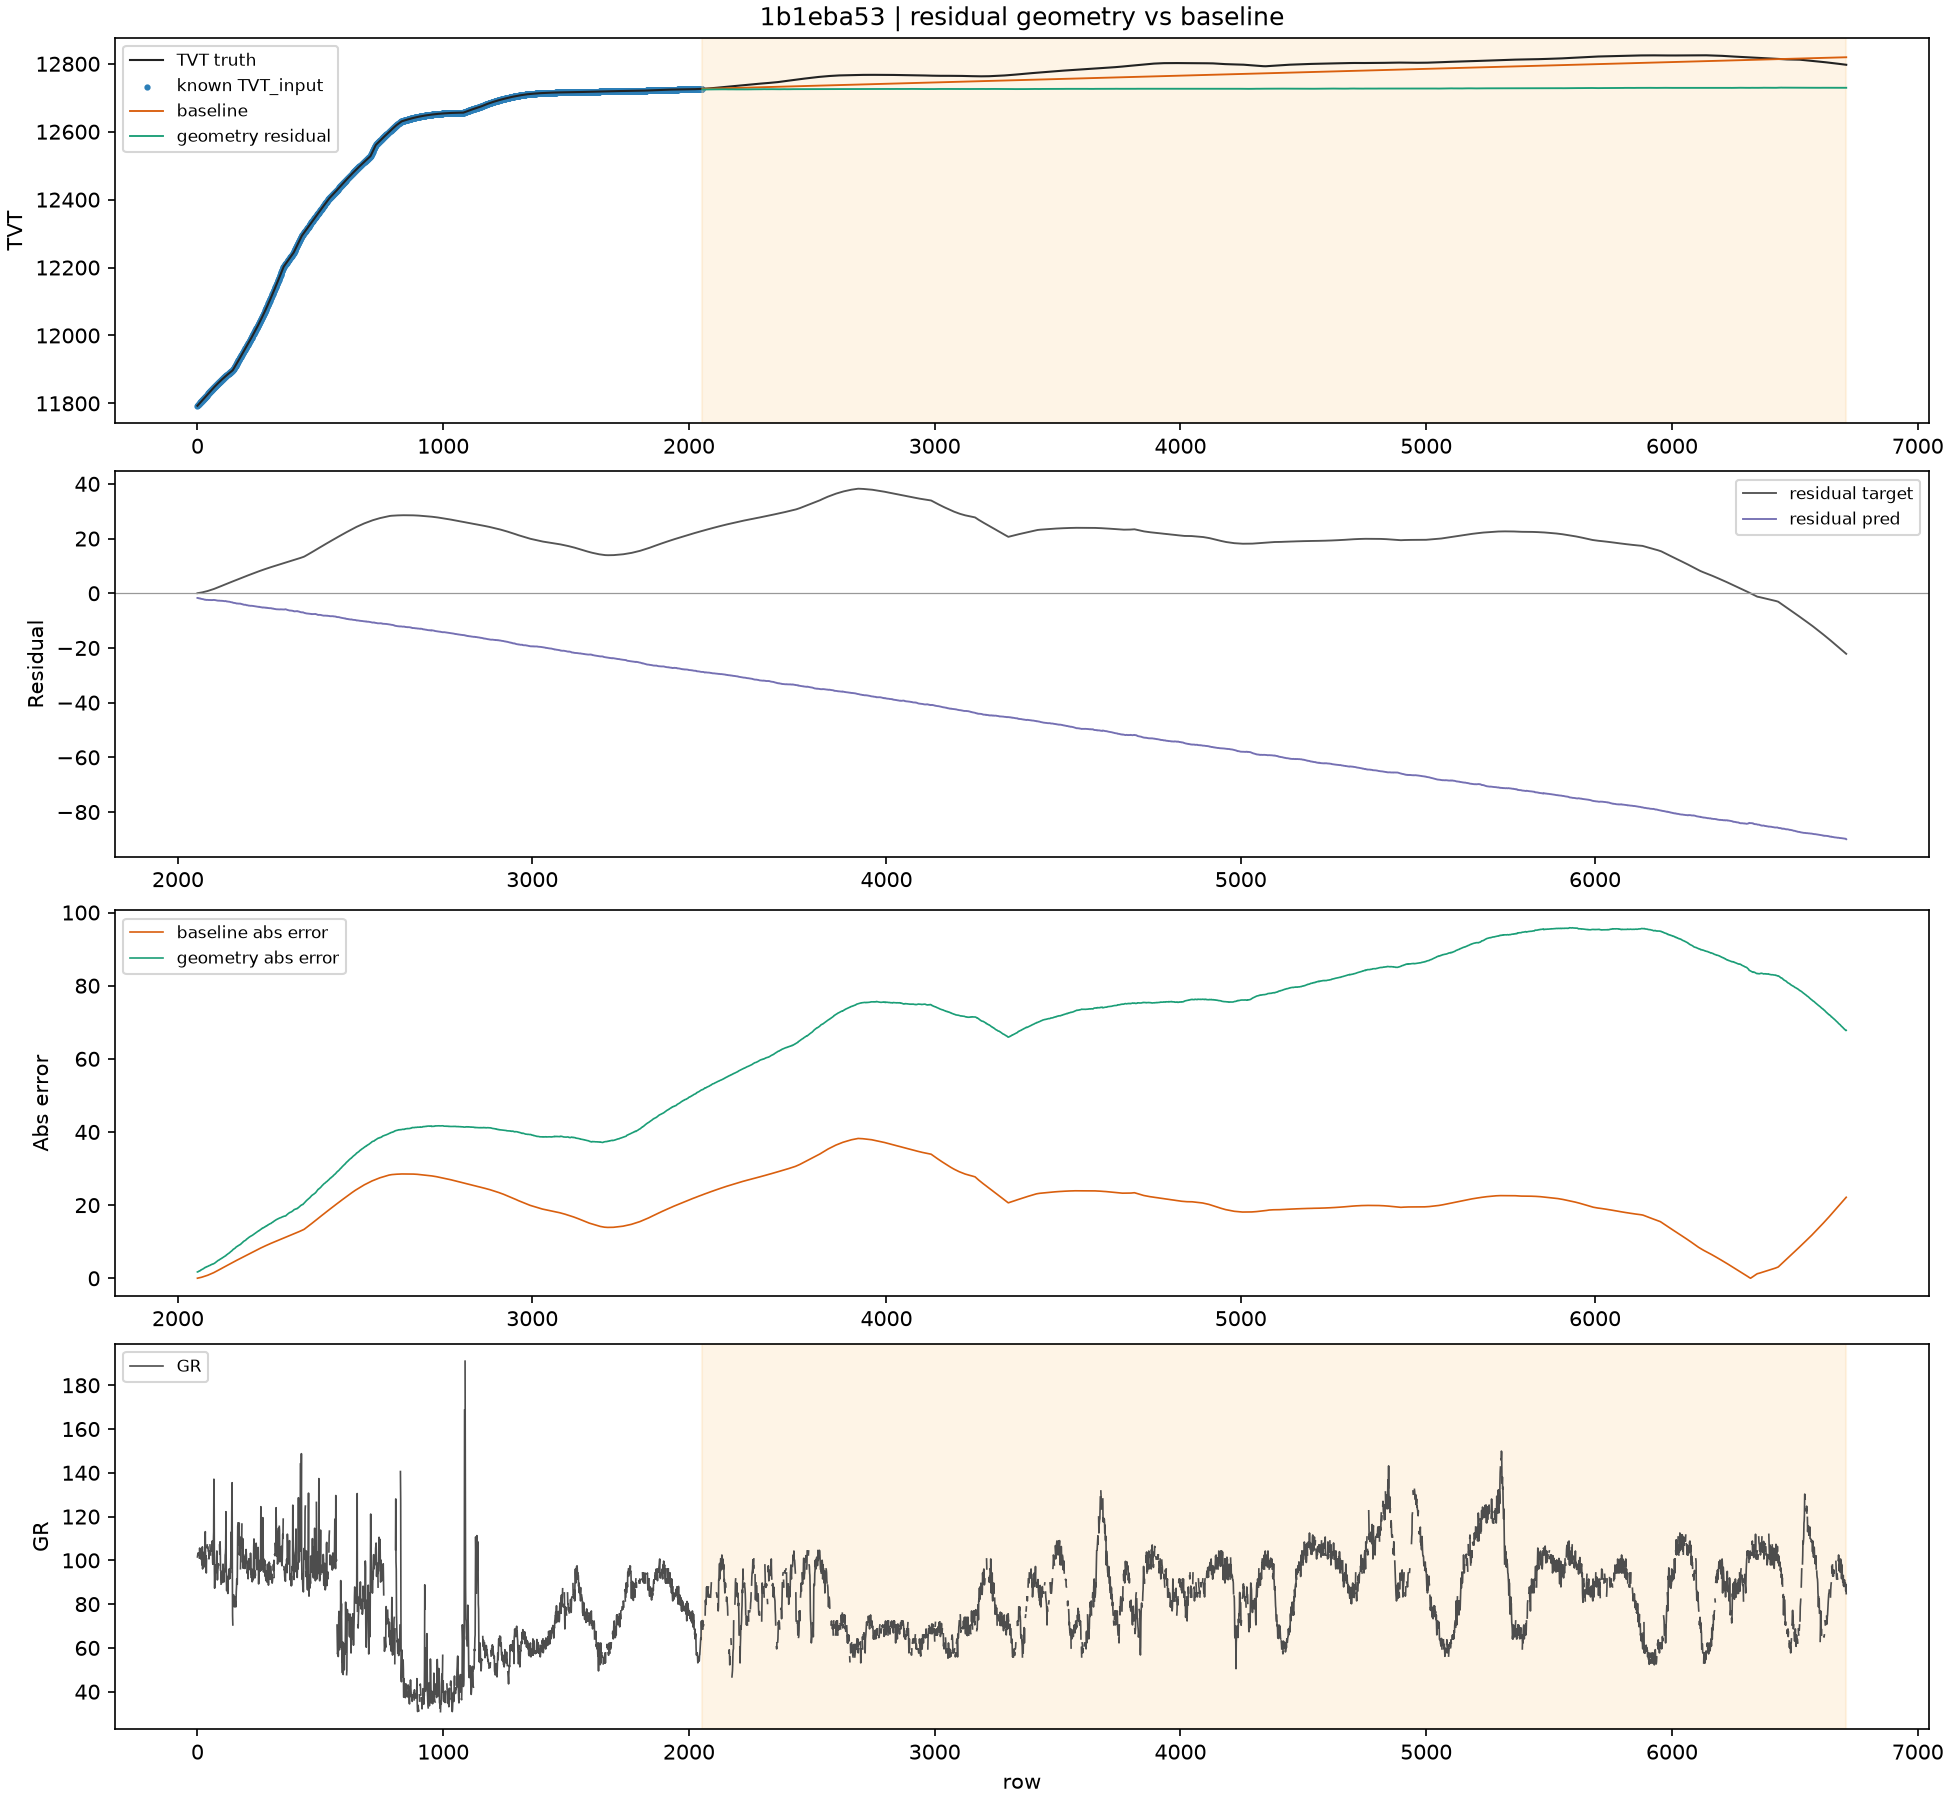
\includegraphics[width=0.95\textwidth,height=0.76\textheight,keepaspectratio]{../../reports/figures/residual_geometry_worst_degraded/01_1b1eba53.png}
\caption{几何残差模型最差退化井示例：`1b1eba53`}
\end{figure}

\end{document}
